\subsection{The F-zkNN Probabilistic Classifier} 
\label{sec:sec_alg}
The F-zkNN probabilistic classifier has been unified in a single distributed session over the Flink framework. Flink offers a variety of \textit{transformations} on datasets and is more flexible due to the fact that a task can be carried out by a number of available generic \textit{task managers}, which mostly denote a single machine on a cluster, constituted of several processing slots. The reduce transformation can be executed over grouped datasets, via the \textit{groupBy} operation, which assigns a part of the dataset to a different reducer, according to a pre-specified field. In order to achieve similar functionality to the Hadoop's map and reduce operations, the \textit{FlatMap} and \textit{GroupReduce} transformations are used, which return an arbitrary number of elements, rather than just a single one. Another aspect that makes Flink more appropriate, is that it does not require key-value pairs during the transitions that take place between the transformations. Instead, \textit{Objects} or just primitive types are used, optionally grouped in \textit{Tuples}. 

The scheme of the proposed algorithm, depicted in Figure~\ref{fig:single_session}, consists of the following three MapReduce stages:

\begin{figure}[htbp]
	\centering
	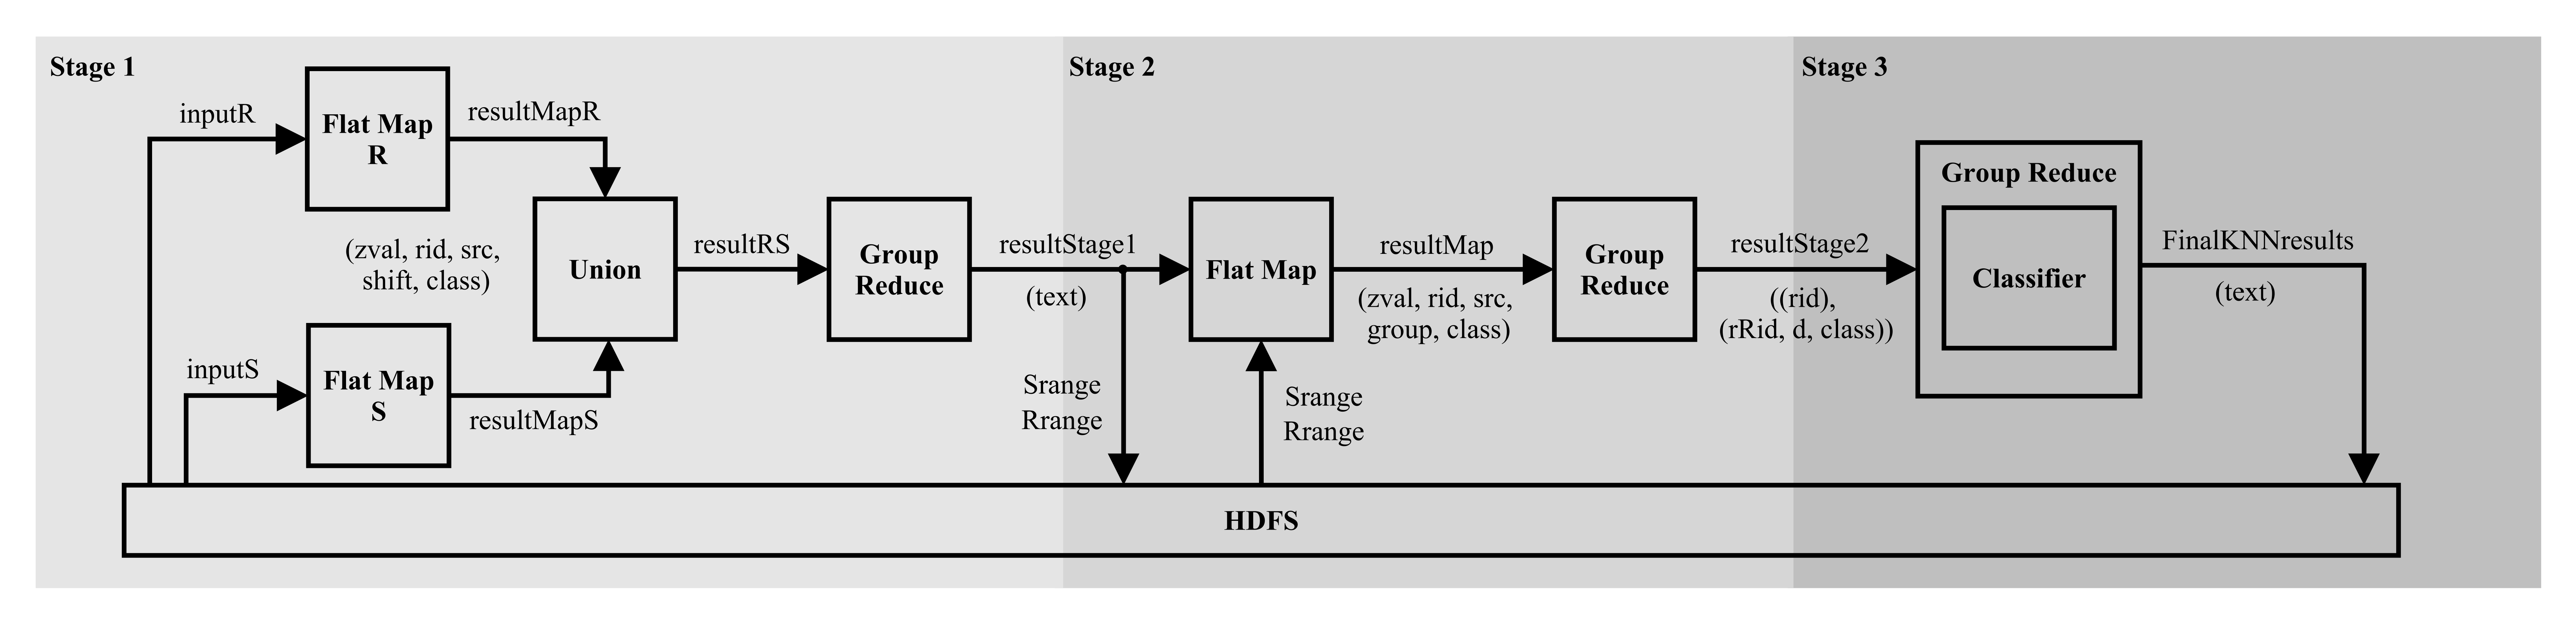
\includegraphics[width=\textwidth]{figures/singlesession.png}
	\caption{Single session F-zkNN.}{}
	\label{fig:singlesession}
\end{figure}

\subsubsection{The pre-processing stage}
\label{subsec:fzknn3_1}
During the pre-processing stage, the $R$ and $S$ datasets, along with the random vectors, are read as plain text from the HDFS and delivered to two separate concurrent FlatMap transformations, identifiable by the input source file. For each of the $\alpha$ number of shifts, (Algorithm~\ref{alg:single_session_algorithm_stage1}, Line 2), the shifted datasets and their $z$-values are calculated (Lines 3 and 4) and passed on a \textit{Union} transformation (Line 5). This results in a union of the two datasets, which is passed (as an object containing the values $(zval, rid, src, shift, class)$) on a GroupReduce transformation, grouped by the shift number. During the reduce phase, the datasets are sampled ($\hat{R_i}$ and $\hat{S_i}$) and cached locally (Lines 5-16). The partition ranges ($Rrange_i$ and $Srange_i$) for each shift are calculated using the sampled datasets and are stored on the HDFS (Lines 17 and 18). The output of this stage is the locally cached transformed datasets, which are finally read from the cache and feed the next stage (Line 19).

\vspace{-2mm}
\begin{algorithm}[htbp]
	\scriptsize
	\DontPrintSemicolon
	%\Comment The preprocessing stage's input \;
	\KwIn{Datasets $R$, $S$ and random vectors $\textbf{V}=\{\textbf{v}_1, ..., \textbf{v}_\alpha\}, \textbf{v}_1=\overrightarrow{0}$}
	%\Comment The output, that will be emitted to the next stage \;
	\KwOut{Transformed datasets $R^T_i$ and $S^T_i, i=1,...,\alpha$}
	\BlankLine
	\Begin{
		%\Comment The same procedure is performed for each shift \;
		\For{$i=1,...,\alpha$}{
			$R_i = R + \textbf{v}_i$, $S_i = S + \textbf{v}_i$ \\
			$R^T_i \leftarrow \proc{calcZval}(R_i)$, $S^T_i \leftarrow \proc{calcZval}(S_i)$ \\
			\ForEach{$x \in R_i \cup S_i$}{
				%\Comment Sampling \;
				$r \leftarrow \proc{Random}(0,1)$\\
				\If{$r < MinThreshold$}{
					\If{$x \in R_i$}{$\proc{InsertSample}(s, \hat{R_i})$}
					\ElseIf{$x \in S_i$}{$\proc{InsertSample}(s, \hat{S_i})$}					
				}
				$\proc{storeLocal}(s)$
			}
			$Rrange_i \leftarrow \proc{calcRange}(\hat{R_i})$, $Srange_i \leftarrow \proc{calcRange}(\hat{S_i})$ \\
			$\proc{storeHDFS}(Rrange_i, Srange_i)$ \\
			%\Comment Emit to the partitioning and pre-calculation stage \;
			\Return $\proc{fetchLocal}(R^T_i, S^T_i)$
		}
	}
	\caption{The F-zkNN pre-processing stage.}
	\label{alg:single_session_algorithm_stage1}	
\end{algorithm}
\vspace{-4mm}

\subsubsection{The partitioning and pre-calculation stage}
\label{subsec:fzknn3_2}
In this stage, the transformed datasets are received by the mappers and the previously computed partition ranges are used (Algorithm~\ref{alg:single_session_algorithm_stage2}, Line 4) to partition the datasets to $n\times\alpha$ blocks, (Lines 8 and 15), $\alpha$ being the number of shifts and $n$ the number of partitions. Each block is then delivered to a different reducer (Lines 19-28) by using the groupBy operation (as an object containing $(zval, rid, src, group, class)$). There, a range search is performed on each sorted partition and the $k$-NN of each $x \in R$ element are determined (Line 22). The neighbouring elements' coordinates are then calculated (Line 23), un-shifted using the random vectors (Line 24) and their distance to the $x \in R$ element is computed (Line 25). Finally, they are integrated into the proper dataset (Line 26) grouped by element, along with the calculated distance and feed the final stage (Line 30).

\vspace{-2mm}
\begin{algorithm}[htbp]
	\scriptsize
	\DontPrintSemicolon
	%\Comment This stage's input are the datasets emitted during the pre-processing stage \;
	\KwIn{Datasets $R^T_i$, $S^T_i$, $i=1,...,\alpha$}
	%\Comment The output, that will be emitted to the next stage \;
	\KwOut{Dataset $R_{kNearest \times \alpha}$}
	\BlankLine
	\Begin{
		%\Comment Initialization of the dataset to be emitted \;
		$R_{kNearest \times \alpha} = \emptyset$ \\
		%\Comment Again, repeat for each shift \; 
		\For{$i=1,...,\alpha$}{
			$\proc{readHDFS}(Rrange_i, Srange_i)$ \\
			%\Comment Partition the $R$ elements \;
			\ForEach{$x \in R^T_i$}{
				\For{$g=1,..., n$}{
					\If{$\proc{zval}(s) \in Rrange_i(g) $}{
						$\proc{addintopartition}(s, R^{g \times i})$
					}
				}
			}
			%\Comment Partition the $S$ elements \;
			\ForEach{$x \in S^T_i$}{
				\For{$g=1,..., n$}{
					\If{$\proc{zval}(s) \in Srange_i(g) $}{
						$\proc{addintopartition}(s, S^{g \times i})$
					}
				}
			}
			\For{$g=1,..., n$}{
				%\Comment Sorting is needed to properly perform range search \;
				$\proc{sort}(R^{g \times i})$, $\proc{sort}(S^{g \times i})$ \\
				\ForEach{$x \in R^{g \times i}$}{
					$RES \leftarrow \proc{rangeSearch}(s, kNearest, S^{g \times i})$ \\
					$CC \leftarrow \proc{calcCoords}(RES)$ \\
					$US \leftarrow \proc{unshift}(CC)$ \\
					$CD \leftarrow \proc{calcDist}(s, US)$ \\
					$R_{kNearest \times \alpha} \leftarrow \proc{add}(s \times CD, R_{kNearest \times \alpha})$
				}
			}		
		}
		%\Comment Emit to the final stage, grouped by element \;
		\Return $R_{kNearest \times \alpha}$	
	}
	\caption{The F-zkNN partitioning and pre-calculation stage.}
	\label{alg:single_session_algorithm_stage2}	
\end{algorithm}
\vspace{-4mm}
	
\subsubsection{The $k$-NN stage}
\label{subsec:fzknn3_3}
In the final stage, we directly propagate the second stage's results to the reducers. This increases the calculation efficiency as it reduces the resource requirements of the execution. Thus, the calculated $\alpha \times k$-NN of each $R$ element, are received in this stage's reducers (Algorithm~\ref{alg:single_session_algorithm_stage3}, Lines 3-7), which perform $|R|$ reduce tasks via a Tuple containing a string value and an object containing $(rid, rRid, d, class)$. The $k$-NN of each $R$ element are fetched from the grouped set of $R_{k \times \alpha}$. After determining its final nearest neighbours (Line 4), each query element is classified (Line 5) according to the probability of each class, which is calculated by using the Equation~\ref{eq:3}. Finally, the results are added to the resulting dataset (Line 6), which is then stored on the HDFS (Line 8).
 
\vspace{-2mm} 
\begin{algorithm}[htbp]
 	\scriptsize
 	\DontPrintSemicolon
 	%\Comment The input is the grouped by element dataset emitted during the previous stage \;
 	\KwIn{Datasets $R, R_{kNearest \times \alpha}$}
 	%\Comment The algorithm's results \;
 	\KwOut{Stored dataset $R_f$ on the HDFS}
 	\BlankLine
 	\Begin{
 		%\Comment Initialization of the final dataset \;
 		$R_f = \emptyset$ \\
 		\ForEach{$x \in R$}{
 			$RES \leftarrow \proc{$k$-NN}(x, R_{kNearest \times i})$ \\
 			$C \leftarrow \proc{classify}(RES)$	\\		
 			$R_f \leftarrow \proc{add}(s, C, R_f)$ \\
 		}
 		%\Comment Store the final results on HDFS \;
 		$\proc{storeHDFS}(R_f)$
 	}
 	\caption{The F-zkNN $k$-NN stage.}
 	\label{alg:single_session_algorithm_stage3}
\end{algorithm}